\documentclass[10pt]{article}
\usepackage[margin=0.9in]{geometry}

\usepackage{microtype}
\usepackage{amsmath,amssymb,amsthm}
\usepackage{booktabs,array}
\usepackage{pgfplots}\pgfplotsset{compat=1.16}
\usepackage{natbib}
\usepackage[colorlinks=true,urlcolor=blue!50!black,linkcolor=black,citecolor=black]{hyperref}
\usepackage{titlesec,enumitem}
\titleformat{\section}{\large\bfseries}{}{0pt}{}
\titlespacing*{\section}{0pt}{9pt}{3pt}
\setlength{\parindent}{0pt}\setlength{\parskip}{4pt}
\theoremstyle{plain}\newtheorem{proposition}{Proposition}
\theoremstyle{remark}\newtheorem*{remark}{Remark}
\newcommand{\E}{\mathbb{E}}
\newcommand{\Var}{\operatorname{Var}}

\begin{document}

\begin{center}
{\Large\bfseries Indonesian Rupiah (USD/IDR): Currency Report}\\[2pt]
{\small 26 October 2026 \quad Spot reference: 18,088 IDR per USD (23 October 2026)}
\end{center}

\section{Summary and Forecast}
We forecast USD/IDR at 18,600 in one year, 18,600 in three and 19,300 in five, from 18,088 on 23 October 2026 (\href{https://databoks.katadata.co.id/en/market/statistics/32ec67c22c32882/rupiah-exchange-rate-weakens-to-idr-180878-per-us-dollar-friday-23-october-2026}{Databoks}). Risks skew toward a weaker rupiah: it is cheap in real terms, but the Fed is hiking, oil is high, and Indonesia's institutions face a credibility shock.

\begin{center}
\small
\begin{tabular}{lrrrr}
\toprule
Horizon & Bull (15\%) & Base (55\%) & Bear (30\%) & Weighted \\
\midrule
1 year  & 17,200 & 18,300 & 19,800 & 18,600 \\
3 years & 16,600 & 17,900 & 21,000 & 18,600 \\
5 years & 16,800 & 18,300 & 22,500 & 19,300 \\
\bottomrule
\end{tabular}\\[2pt]
{\footnotesize Rupiah per dollar; higher is weaker.}
\end{center}

\section{Fundamentals and Regime}
Indonesia is not in recession; the pressure is external and institutional. GDP grew 5.29\% in Q2 2026 (\href{https://en.antaranews.com/news/425619/manufacturing-consumption-drive-indonesias-529-percent-q2-growth}{Antara}). September CPI of 3.28\% is inside BI's $2.5\pm1\%$ target and below US CPI of 3.7\%, so the 2026 slide is a real depreciation and a rising risk premium, not an inflation story (\href{https://www.bi.go.id/en/publikasi/ruang-media/news-release/Pages/sp_2823326.aspx}{BI}, \href{https://forexfundamentals.com/economic-calendar/us-cpi/2026-10-14}{US CPI}).

The weak spots are external and fiscal. The Q2 current account deficit hit USD 12.5bn (3.3\% of GDP) on a USD 10.2bn oil deficit (\href{https://www.bi.go.id/en/publikasi/ruang-media/news-release/Pages/sp_2816526.aspx}{BI}). The 2026 budget deficit is tracking 2.85\% of GDP against a 3\% cap (\href{https://english.kontan.co.id/news/indonesias-2026-budget-deficit-outlook-seen-at-285-of-gdp-house-panel-says}{Kontan}), BI has revived bond ``burden sharing'' (\href{https://www.indoneo.com/capital/indonesia-central-bank-burden-sharing-deficit-breach/}{Indoneo}), and Moody's and Fitch have negative outlooks. Reserves of USD 146.3bn are the main buffer. The regime is a managed float: BI sets the rate (5.75\%), intervenes in spot and NDF markets, and sells high-yield SRBI bills, 27\% of them foreign-held.

\section{Recent Events}
Three shocks overlapped in 2026. Oil spiked on the Iran war, and the Fed hiked to 3.75--4.00\% in September (\href{https://www.usbank.com/investing/financial-perspectives/market-news/federal-reserve-interest-rate.html}{U.S.\ Bank}). Domestically, BI hiked 100 bp between May and June (\href{https://www.bi.go.id/en/publikasi/ruang-media/news-release/Pages/sp_2810726.aspx}{BI}), parliament added a growth mandate to BI's objectives in June (\href{https://www.rajahtannasia.com/?p=193848}{Rajah \& Tann}), and Governor Warjiyo resigned in July (\href{https://kuwaittimes.com/article/49022/business/indonesia-names-new-central-bank-governor/}{Kuwait Times}). On 15--16 October MSCI proposed demoting Indonesia to ``standalone'' status, stocks fell 11.6\% and the rupiah hit a record near 18,050 (\href{https://coinpedia.org/news/indonesia-stocks-crash-11-6-as-msci-threat-sends-rupiah-to-record-low/}{Coinpedia}). BI held at 5.75\% on 21 October but cut reserve requirements.

\section{Forecast Rationale}
\textbf{Short term: flows dominate.} The MSCI decision (due by 30 June 2027) and further Fed hikes keep the risk premium high, while carry and reserves limit the slide. Base case 18,300; a downgrade plus more hikes gives 19,800. The weighted 18,600 equals the carry-implied forward, so holding rupiah offers no edge.

\textbf{Medium term: valuation pulls.} The rupiah is about 28\% below its 2005--2025 real average and Indonesian inflation is below US inflation. As the oil deficit unwinds the base case recovers to 17,900. Reversion is slow (half-life of 5 to 9 years), so the 19,100--19,700 forward overstates depreciation and rupiah carry should pay.

\textbf{Long term: the anchor is institutional.} With both countries targeting low inflation, drift falls to about 0.5\% a year (base 18,300). The bear case (22,500) is regime change: a growth mandate plus a breached deficit rule turn burden sharing into monetization.

\textbf{Risks.} Weaker: oil above USD 110, an MSCI downgrade, a fiscal breach. Stronger: a ceasefire, free-float reforms, a Fed pause.

\newpage
\section*{Appendix: Methods and Formal Results}
\textbf{Data and notation.} $S_t$ is USD/IDR (higher means a weaker rupiah), built from ECB euro reference rates, April 2005 to September 2026, with later spot from Databoks. $P_t$ and $P_t^*$ are Indonesian and US price levels from World Bank, BPS and BLS CPI. The log real rate is $q_t=\ln S_t+\ln P_t^*-\ln P_t$, with sample mean $\bar q$ over 2005--2025. Policy rates are $i=5.75\%$ (BI-Rate), $i_{\mathrm{SRBI}}=6.94\%$ (12-month SRBI, 11 September 2026 auction) and $i^*=3.875\%$ (Fed funds midpoint).

\begin{figure}[h]
\centering
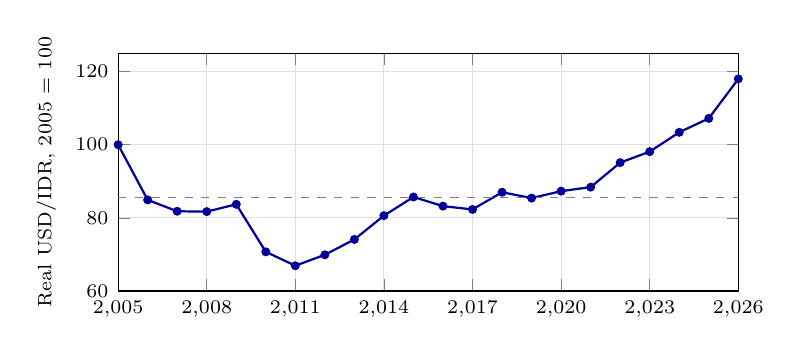
\begin{tikzpicture}
\begin{axis}[width=0.78\textwidth,height=4.6cm,xlabel={},ylabel={Real USD/IDR, 2005 = 100},
 xmin=2005,xmax=2026,ymin=60,ymax=125,tick label style={font=\scriptsize},label style={font=\scriptsize},
 xtick={2005,2008,2011,2014,2017,2020,2023,2026},grid=major,grid style={gray!25}]
\addplot[blue!60!black,thick,mark=*,mark size=1.2pt] coordinates {
(2005,100.0)(2006,84.9)(2007,81.8)(2008,81.7)(2009,83.7)(2010,70.7)(2011,66.9)(2012,69.9)(2013,74.1)(2014,80.6)(2015,85.7)(2016,83.2)(2017,82.3)(2018,87.0)(2019,85.4)(2020,87.3)(2021,88.4)(2022,95.1)(2023,98.1)(2024,103.4)(2025,107.2)(2026,118.0)};
\addplot[gray,dashed] coordinates {(2005,85.6)(2026,85.6)};
\end{axis}
\end{tikzpicture}\\[-2pt]
{\scriptsize Figure 1. Real USD/IDR (CPI-deflated); dashed line is the 2005--2025 mean (86). 2026 uses 23 October spot and CPI through September.}
\end{figure}

\begin{proposition}[Real-rate reversion]
Suppose $x_t=q_t-\bar q$ follows $x_{t+1}=\rho x_t+\varepsilon_{t+1}$ with $|\rho|<1$ and $\E[\varepsilon_{t+1}\mid\mathcal F_t]=0$. Then $\E_t[x_{t+h}]=\rho^h x_t$, and the half-life is $\tau=\ln(1/2)/\ln\rho$.
\end{proposition}
\begin{proof}
Iterating, $x_{t+h}=\rho^h x_t+\sum_{k=1}^{h}\rho^{h-k}\varepsilon_{t+k}$. Taking $\E_t$ kills the sum. Setting $\rho^\tau=\tfrac12$ gives $\tau$. \qedhere
\end{proof}
\textit{Application.} Estimated $\hat\rho=0.876$ (s.e.\ 0.139) on annual data and $0.994$ (HAC s.e.\ 0.011) on monthly data, giving $\tau=5.2$ and $9.0$ years. An ADF test on monthly $q_t$ fails to reject a unit root ($p=0.77$), the PPP puzzle \citep{rogoff1996,lothian1996}. Today $x_t=\ln(1.389)=0.328$, so with $\tau=9.0$ the PPP-implied path is 17,650, 16,900 and 16,280 at 1, 3 and 5 years with no inflation gap (17,740, 17,150 and 16,690 with a 0.5 pp gap). The base cases in the table sit above this path because PPP is only a pull, and the sample mean includes the 2010--2012 commodity boom.

\begin{proposition}[Carry-implied forward]
If covered interest parity holds at horizon $h$ years with annualised rates $i$ and $i^*$, then $F_{t,h}=S_t\left(\dfrac{1+i}{1+i^*}\right)^{h}$. A dollar-funded investor long rupiah earns an expected excess return $\lambda=\E_t\!\left[\ln\dfrac{S_t}{S_{t+h}}\right]+h\ln\dfrac{1+i}{1+i^*}$, which is zero under UIP and equals the risk premium otherwise.
\end{proposition}
\begin{proof}
Borrowing one dollar buys $1/S_t$ rupiah, which grow to $(1+i)^h/S_t$ and convert back at $S_{t+h}$. No arbitrage fixes $S_{t+h}=F_{t,h}$ for a hedged position, so $F_{t,h}=S_t\left(\frac{1+i}{1+i^*}\right)^{h}$. Taking logs of the unhedged payoff relative to the dollar loan gives $\lambda$. \qedhere
\end{proof}
\textit{Application.} With the BI-Rate the forwards are 18,414, 19,085 and 19,780 at 1, 3 and 5 years; with the SRBI yield, 18,621, 19,736 and 20,917. UIP fails \citep{fama1984}: in October 2025 the rate gap was under 1 pp, yet USD/IDR rose 8.9\% over the year. EM premia track local policy uncertainty \citep{kalemli2026}, and carry earns positive average excess returns at the price of crash risk \citep{lustig2007,brunnermeier2008}, which is why the weighted 3- and 5-year forecasts sit below the forward.

\begin{proposition}[Intermediation and flow pricing]
Let risk-averse intermediaries with mean-variance preferences (risk aversion $\gamma$) absorb net dollar demand $f_t$ not met by central bank supply $x_t$, and let $\sigma_t^2=\Var_t(\ln S_{t+1})$. Then $\ln S_t-\ln S_t^{\mathrm{UIP}}=\Gamma_t\,(f_t-x_t)$ with $\Gamma_t=\gamma\sigma_t^2$.
\end{proposition}
\begin{proof}
Intermediaries hold $D_t=f_t-x_t$ rupiah. Their one-period excess return per unit is $\lambda_t=(i-i^*)-\E_t[\Delta\ln S_{t+1}]$. Maximising $D\lambda_t-\tfrac{\gamma}{2}D^2\sigma_t^2$ gives $D_t=\lambda_t/(\gamma\sigma_t^2)$. Market clearing then gives $\lambda_t=\gamma\sigma_t^2(f_t-x_t)$. Substituting $\lambda_t$ and rearranging, $\ln S_t=\E_t\ln S_{t+1}-(i-i^*)+\Gamma_t(f_t-x_t)$, so the deviation from the UIP price is $\Gamma_t(f_t-x_t)$. \qedhere
\end{proof}
\textit{Application.} This is a stylised reduced form of \citet{gabaix2015}. It implies that MSCI-related outflows (Goldman estimates USD 5.6bn) move the rupiah with fundamentals unchanged, that BI's DNDF, NDF and SRBI operations work by lowering $f_t-x_t$ \citep{fanelli2021,itskhoki2023}, and that higher volatility raises $\Gamma_t$. Weaker monetary credibility also raises local-currency bond risk \citep{du2020}, consistent with the 10-year yield rising from 6.03\% to 7.37\% between end-2025 and July 2026 (\href{https://www.idnfinancials.com/news/66794/dbs-indonesias-10-year-yield-unlikely-to-fall-below-7}{IDN Financials}).

\textbf{Volatility and regime.} A GARCH(1,1) with Student-$t$ errors on daily log returns gives $\hat\alpha=0.136$, $\hat\beta=0.864$, $\hat\nu=4.0$, so volatility shocks are near-permanent and tails are fat. Scenario bands therefore use overlapping 12-, 36- and 60-month changes since 2005, whose de-meaned 80\% ranges are $-8.6/+9.4\%$, $-14.3/+21.3\%$ and $-17.9/+22.6\%$; the bull and bear cases lie inside them. In 2026, 89\% of monthly moves stayed within 2\% and realised volatility was 5.4\% against 8.3\% historically, a de facto crawling band \citep{reinhart2004} and fear of floating \citep{calvo2002}.

\textbf{Event study.} Three-day returns scaled by GARCH volatility (positive means a weaker rupiah): P2SK amendment (17 June 2026) $+0.85\%$, $z=0.80$; Warjiyo resignation (27 July) $+0.74\%$, $z=1.16$; BI off-cycle hike (9 June) $-0.92\%$, $z=-1.33$; MSCI first warning (28 January) $+0.01\%$, $z=0.01$. None is significant at 5\%: daily fixings are too coarse, and identification needs intraday data \citep{gurkaynak2005,nakamura2018}.

\begingroup\footnotesize
\begin{thebibliography}{99}\setlength{\itemsep}{0pt}\setlength{\parskip}{0pt}
\bibitem[Brunnermeier et al.(2008)]{brunnermeier2008} Brunnermeier, Nagel, Pedersen (2008). Carry trades and currency crashes. \textit{NBER Macroeconomics Annual} 23.
\bibitem[Calvo and Reinhart(2002)]{calvo2002} Calvo, Reinhart (2002). Fear of floating. \textit{QJE} 117(2).
\bibitem[Du et al.(2020)]{du2020} Du, Pflueger, Schreger (2020). Sovereign debt portfolios, bond risks, and the credibility of monetary policy. \textit{J.\ Finance} 75(6).
\bibitem[Fama(1984)]{fama1984} Fama (1984). Forward and spot exchange rates. \textit{J.\ Monetary Econ.} 14(3).
\bibitem[Fanelli and Straub(2021)]{fanelli2021} Fanelli, Straub (2021). A theory of foreign exchange interventions. \textit{Rev.\ Econ.\ Stud.} 88(6).
\bibitem[Gabaix and Maggiori(2015)]{gabaix2015} Gabaix, Maggiori (2015). International liquidity and exchange rate dynamics. \textit{QJE} 130(3).
\bibitem[G\"urkaynak et al.(2005)]{gurkaynak2005} G\"urkaynak, Sack, Swanson (2005). Do actions speak louder than words? \textit{Int.\ J.\ Central Banking} 1(1).
\bibitem[Itskhoki and Mukhin(2023)]{itskhoki2023} Itskhoki, Mukhin (2023). Optimal exchange rate policy. NBER working paper.
\bibitem[Kalemli-{\"O}zcan and Varela(2026)]{kalemli2026} Kalemli-\"Ozcan, Varela (2026). \href{https://www.nber.org/papers/w28923}{Five facts about the UIP premium}. \textit{NBER ISOM 2026}; NBER WP 28923.
\bibitem[Lothian and Taylor(1996)]{lothian1996} Lothian, Taylor (1996). Real exchange rate behavior. \textit{JPE} 104(3).
\bibitem[Lustig and Verdelhan(2007)]{lustig2007} Lustig, Verdelhan (2007). The cross section of foreign currency risk premia and consumption growth risk. \textit{AER} 97(1).
\bibitem[Nakamura and Steinsson(2018)]{nakamura2018} Nakamura, Steinsson (2018). High-frequency identification of monetary non-neutrality. \textit{QJE} 133(3).
\bibitem[Reinhart and Rogoff(2004)]{reinhart2004} Reinhart, Rogoff (2004). The modern history of exchange rate arrangements. \textit{QJE} 119(1).
\bibitem[Rogoff(1996)]{rogoff1996} Rogoff (1996). The purchasing power parity puzzle. \textit{J.\ Econ.\ Literature} 34(2).
\end{thebibliography}
\endgroup

\end{document}
